\documentclass[a4paper,11pt]{report}
\usepackage[showexo=true,showcorr=false]{../packages/coursclasse}
%Commenter ou enlever le commentaire sur la ligne suivante pour montrer le niveau
\toggletrue{montrerNiveaux}
%permet de gérer l'espacement entre les items des env enumerate et enumitem
\usepackage{enumitem}
\setlist[enumerate]{align=left,leftmargin=1cm,itemsep=10pt,parsep=0pt,topsep=0pt,rightmargin=0.5cm}
\setlist[itemize]{align=left,labelsep=1em,leftmargin=*,itemsep=0pt,parsep=0pt,topsep=0pt,rightmargin=0cm}
%permet de gerer l'espacement entre les colonnes de multicols
\setlength\columnsep{20pt}


\begin{document}

%%%%%%%%%%%%%%%%% À MODIFIER POUR CHAQUE SERIE %%%%%%%%%%%%%%%%%%%%%%%%%%%%%
\newcommand{\chapterName}{Espace}
\newcommand{\serieName}{Construction des quadrilatères}


%%%%%%%%%%%%%%%%%% PREMIERE PAGE NE PAS MODIFER %%%%%%%%%%%%%%%%%%%%%%%%
% le chapitre en cours, ne pas changer au cours d'une série
\chapter*{\chapterName}
\thispagestyle{empty}

%%%%% LISTE AIDE MEMOIRE %%%%%%
\begin{amL}{\serieName}{
\item Tracer la droite perpendiculaire à une droite donnée passant par un point donné (page 93)
\item Tracer la droite parallèle à une droite donnée passant par un point donné (page 95)
\item Quadrilatère (page 123)
\item Quadrilatères particuliers (pages 123-124)
}
\end{amL}

%%%%%%%%%%%%%%% DEBUT DE LA SERIE NE PAS MODIFIER %%%%%%%%%%%%%%%%%%%%%%%%%%%%%
\section*{\serieName}
\setcounter{page}{1}
\thispagestyle{firstPage}



%%%%%%%%%%% LES EXERCICES %%%%%%%%%%%%%%%%%%%%%%%%%%%%%%%%%%%%



\begin{exo}{
Les dessins suivants sont des croquis. Construis-les en respectant les mesures et les codages indiqués.
\begin{tasks}(2)
    \task ~\\ 

\begin{tikzpicture}

{\scriptsize
\coordinate[](A) at (0,0);
\coordinate[](B) at (2,0);
\coordinate[](C) at (2,4);
\coordinate[](D) at (0,4);

\tkzMarkRightAngle(A,B,C) ;
\tkzMarkRightAngle(B,C,D) ;
\tkzMarkRightAngle(C,D,A) ;
\tkzMarkRightAngle(D,A,B) ;

\draw (A)-- (B) -- (C) -- (D) -- cycle;

\draw[<->, >=latex] (2.5,0) -- (2.5,4);
\node[right] at (2.5,2) {5,2 cm} ;

\draw[<->, >=latex] (2,4.5) --node[above]{$\tunit{4,1}{\cm}$} (0,4.5) ;
%\node[above] at (1,4.5) {4,7 cm} ;


\draw[dotted] (B) -- ++(0.5,0) ;
\draw[dotted] (C) -- ++(0.5,0) ;
\draw[dotted] (D) -- ++(0,0.5) ;
\draw[dotted] (C) -- ++(0,0.5) ;

\node[below left] at (A) {$A$};
\node[below right] at (B) {$B$};
\node[above right] at (C) {$C$};
\node[above left] at (D) {$D$};
}

\end{tikzpicture}

    \task ~\\ 

\begin{tikzpicture}

{\scriptsize
\coordinate[](E) at (0,0);
\coordinate[](F) at (3,0);
\coordinate[](G) at (3,3);
\coordinate[](H) at (0,3);

\tkzMarkRightAngle(E,F,G) ;
\tkzMarkRightAngle(F,G,H) ;
\tkzMarkRightAngle(G,H,E) ;
\tkzMarkRightAngle(H,E,F) ;

\draw (E)--node[sloped]{$//$} (F) --node[]{$//$} (G) --node[sloped]{$//$} (H) --node[]{$//$} cycle;

\draw[<->, >=latex] (3.5,0) --node[right]{$$\tunit{3,7}{\cm}$$} (3.5,3);


\draw[dotted] (G) -- ++(0.5,0);
\draw[dotted] (F) -- ++(0.5,0);
%\node[sloped] at (1.5,0) {$//$} ;
%\node[sloped] at (3,1.5) {$//$} ;
%\node[sloped] at (0,1.5) {$//$} ;
%\node[sloped] at (1.5,3) {$//$} ;

\node[below left] at (E) {$E$};
\node[below right] at (F) {$F$};
\node[above right] at (G) {$G$};
\node[above left] at (H) {$H$};
}

\end{tikzpicture}

\end{tasks}
}{1}
\end{exo}



\begin{exof}{ES79}{134}{1}
\end{exof}
\begin{exof}{ES80}{135}{1}
\end{exof}


\begin{exop}{
Termine la construction des quadrilatères ci-dessous. Utilise tes instruments de géométrie.
\begin{tasks}(2)
    \task parallélogramme \vspace{1cm}\\
    
        \begin{tikzpicture}
        \begin{scope}[rotate=10]
            \draw (0,0) -- (4,0) -- (5,2) ;
        \end{scope}
        \end{tikzpicture}
        
    \task trapèze isocèle \vspace{1cm}\\
    
        \begin{tikzpicture}
        \begin{scope}[rotate=-10]
            \draw (0,0) -- (5,0) -- (4,2) ;
        \end{scope}
        \end{tikzpicture}
    
    \task losange \vspace{2.4cm}\\
    
        \begin{tikzpicture}
        \begin{scope}[rotate=10]
            \draw (-3,1) -- (0,0) -- (3,1) ;
        \end{scope}
        \end{tikzpicture}
        
    \task rectangle \vspace{1cm}\\

        \begin{tikzpicture}
        \begin{scope}[rotate=170]
            \draw (0,0) -- (3,0) -- (3,-2) ;
        \end{scope}
        \end{tikzpicture}
        
\end{tasks}
}{1}
\end{exop}


\begin{exop}{
Termine la construction des quadrilatères ci-dessous. Utilise tes instruments de géométrie.
\begin{tasks}(2)
    \task parallélogramme \vspace{0.5cm}\\
    
        \begin{tikzpicture}
        \begin{scope}[rotate=190]
            \draw (0,0) -- (3,0) -- (5,2) ;
        \end{scope}
        \end{tikzpicture}
        
    \task trapèze isocèle \vspace{0.5cm}\\
    
        \begin{tikzpicture}
        \begin{scope}[rotate=-190]
            \draw (0,0) -- (4,0) -- (3,3) ;
        \end{scope}
        \end{tikzpicture}
    
    \task losange \vspace{1cm}\\
    
        \begin{tikzpicture}
        \begin{scope}[rotate=10]
            \draw (3,1) -- (0,0) -- (3,-1) ;
        \end{scope}
        \end{tikzpicture}
        
    \task rectangle \vspace{1cm}\\

        \begin{tikzpicture}
        \begin{scope}[rotate=250]
            \draw (0,0) -- (5,0) -- (5,-2) ;
        \end{scope}
        \end{tikzpicture}
        
\end{tasks}
}{1}
\end{exop}



\begin{exop}{
Construis les carrés dont voici les diagonales. Utilise tes instruments de géométrie.

\begin{tasks}(2)
    \task ~\vspace{2cm} \\
    
        \begin{tikzpicture}
        \draw (0,0) -- (3,1) ;
        \end{tikzpicture}
    
    \task ~\vspace{1cm} \\
    
        \hspace{3cm}
        \begin{tikzpicture}
        \draw (0,0) -- (0,4) ;
        \end{tikzpicture}
\end{tasks}
%\begin{center}
%\begin{tikzpicture}
%    \draw (0,0) -- (3,1) ;
%\end{tikzpicture}
%\end{center}

\vspace{2cm}

}{1}
\end{exop}


\begin{exop}{
\begin{tasks}(2)
\task Construis le rectangle $MNOP$ tel que le côté $MN$ mesure le triple du côté $PM$. \vspace{1cm} \\
        \begin{tikzpicture}
            \draw (0,0) -- (1,2) ;
            \node at (-0.4,-0.4) {$M$} ;
            \node at (0.6,2.2) {$P$} ;
        \end{tikzpicture}
\vspace{3cm}

\task Construis le rectangle $ABCD$ tel que le côté $AD$ mesure le double du côté $AB$. \vspace{1cm} \\
        \begin{tikzpicture}
            \draw (0,0) -- (6,1) ;
            \node[above left] at (0,0) {$A$} ;
            \node[above right] at (6,1) {$D$} ;
        \end{tikzpicture}
\vspace{3cm}
\end{tasks}
}{1}
\end{exop}



\begin{exo}{
Construis un losange dont les diagonales mesurent\ldots
\begin{tasks}(2)
    \task \ldots \tunit{5}{\cm} et \tunit{7}{\cm}.
    \task \ldots \tunit{3}{\cm} et \tunit{4}{\cm}.
    \task \ldots \tunit{3,1}{\cm} et \tunit{8,6}{\cm}.
    \task \ldots \tunit{9,5}{\cm} et \tunit{9,5}{\cm}.
\end{tasks}
}{1}
\end{exo}


%\begin{exo}{
%Place trois points $R$, $E$ et $V$ non alignés. Trace à main levée tous les parallélogrammes ayant $R$, $E$ et $V$ comme sommets.
%}{2}
%\end{exo}


\begin{exo}{
Construis les parallélogrammes en respectant les mesures et les codages indiqués sur le croquis. Utilise tes instruments de géométrie.
\begin{tasks}(2)
    \task 

\begin{tikzpicture}
\begin{scope}[rotate=-15]
{\scriptsize
\coordinate[](A) at (0,0);
\coordinate[](B) at (3,0);
\coordinate[](C) at (2,2);
\coordinate[](D) at (-1,2);

\node[below left] at (A) {$A$};
\node[below right] at (B) {$B$};
\node[above right] at (C) {$C$};
\node[above left] at (D) {$D$};

\draw (A)-- (B) -- (C) -- (D) -- cycle;

%angle
\pic [draw, -, "$\ang{50}$", angle eccentricity=1.5]{angle = C--B--A};

\draw[dotted] (B) -- ++(0.5,0) ;
\draw[dotted] (C) -- ++(0.5,0) ;
\draw[<->, >=latex] (3.5,0) --node[right]{$\tunit{3}{\cm}$} (2.5,2);
%\node[right] at (3, 1) {3 cm} ;

\draw[dotted] (D) -- ++(0,0.5) ;
\draw[dotted] (C) -- ++(0,0.5) ;
\draw[<->, >=latex] (-1,2.5) --node[above]{$\tunit{4}{\cm}$} (2,2.5) ;
%\node[above] at (0.5,2.5) {4 cm} ;



}
\end{scope}
\end{tikzpicture}


    \task  

\begin{tikzpicture}

\begin{scope}[rotate=10]
{\scriptsize
\coordinate[](A) at (0,0);
\coordinate[](B) at (2,0);
\coordinate[](C) at (3,4);
\coordinate[](D) at (1,4);

\node[below left] at (A) {$A$};
\node[below right] at (B) {$B$};
\node[above right] at (C) {$C$};
\node[above left] at (D) {$D$};

\draw (A)-- (B) -- (C) -- (D) -- cycle;

%angle
\pic [draw, -, "$\ang{105}$", angle eccentricity=1.5]{angle = C--B--A};

\draw[dotted] (A) -- ++(-0.5,0) ;
\draw[dotted] (D) -- ++(-0.5,0) ;
\draw[<->, >=latex] (-0.5,0) --node[left]{$\tunit{5}{\cm}$} (0.5,4);

\draw[dotted] (A) -- ++(0,-0.5) ;
\draw[dotted] (B) -- ++(0,-0.5) ;
\draw[<->, >=latex] (0,-0.5) --node[below]{$\tunit{2,5}{\cm}$} (2,-0.5) ;



}
\end{scope}
\end{tikzpicture}


    \task 

\begin{tikzpicture}

\begin{scope}[rotate=20]
{\scriptsize
\coordinate[](A) at (0,0);
\coordinate[](B) at (5,0);
\coordinate[](C) at (6,4);
\coordinate[](D) at (1,4);

\node[below left] at (A) {$A$};
\node[below right] at (B) {$B$};
\node[above right] at (C) {$C$};
\node[above left] at (D) {$D$};

\draw (A)-- (B) -- (C) -- (D) -- cycle;

%angle
\pic [draw, -, "$\ang{75}$", angle eccentricity=1.5]{angle = C--B--A};

\draw[dotted] (A) -- ++(-0.5,0) ;
\draw[dotted] (D) -- ++(-0.5,0) ;
\draw[<->, >=latex] (-0.5,0) --node[left]{$\tunit{5}{\cm}$} (0.5,4);

\draw[dotted] (A) -- ++(0,-0.5) ;
\draw[dotted] (B) -- ++(0,-0.5) ;
\draw[<->, >=latex] (0,-0.5) --node[below]{$\tunit{7,3}{\cm}$} (5,-0.5) ;



}\end{scope}

\end{tikzpicture}


    \task  

\begin{tikzpicture}

\begin{scope}[rotate=-10]
{\scriptsize
\coordinate[](A) at (0,0);
\coordinate[](B) at (2,0);
\coordinate[](C) at (1,3);
\coordinate[](D) at (-1,3);

\node[below left] at (A) {$A$};
\node[below right] at (B) {$B$};
\node[above right] at (C) {$C$};
\node[above left] at (D) {$D$};

\draw (A)-- (B) -- (C) -- (D) -- cycle;

%angle
\pic [draw, -, "$\ang{60}$", angle eccentricity=1.5]{angle = B--A--D};

\draw[dotted] (B) -- ++(0.5,0) ;
\draw[dotted] (C) -- ++(0.5,0) ;
\draw[<->, >=latex] (2.5,0) --node[right]{$\tunit{3,2}{\cm}$} (1.5,3);

\draw[dotted] (A) -- ++(0,-0.5) ;
\draw[dotted] (B) -- ++(0,-0.5) ;
\draw[<->, >=latex] (0,-0.5) --node[below]{$\tunit{4,8}{\cm}$} (2,-0.5) ;
}
\end{scope}
\end{tikzpicture}

    
\end{tasks}

}{1}
\end{exo}

\newpage
\begin{exo}{
Construis les trapèzes isocèles en respectant les mesures et les codages indiqués sur le croquis. Utilise tes instruments de géométrie.

\begin{tasks}(2)
    \task ~\\ 


\begin{tikzpicture}

{\scriptsize
\coordinate[](A) at (1,0);
\coordinate[](B) at (4,0);
\coordinate[](C) at (5,3);
\coordinate[](D) at (0,3);

\node[below left] at (A) {$A$};
\node[below right] at (B) {$B$};
\node[above right] at (C) {$C$};
\node[above left] at (D) {$D$};

\pic [draw, -, "$\ang{60}$", angle eccentricity=1.5]{angle = D--C--B};


\draw (A)-- (B) -- (C) -- (D) -- cycle;

\draw[dotted] (A) -- ++(0,-0.5) ;
\draw[dotted] (B) -- ++(0,-0.5) ;
\draw[<->, >=latex] (1,-0.5) --node[below]{$\tunit{2,5}{\cm}$} (4,-0.5);

\draw[dotted] (C) -- ++(0,0.5) ;
\draw[dotted] (D) -- ++(0,0.5) ;
\draw[<->, >=latex] (5,3.5) --node[above]{$\tunit{5,5}{\cm}$} (0,3.5);

\draw[dotted] (A) -- ++(-0.5,0) ;
\draw[dotted] (D) -- ++(-0.5,0) ;
\draw[<->, >=latex] (0.5,0) --node[left]{$\tunit{3,5}{\cm}$} (-0.5,3) ;




}

\end{tikzpicture}


    \task ~\\ \begin{tikzpicture}

\begin{scope}[rotate=190]
{\scriptsize
\coordinate[](A) at (1,0);
\coordinate[](B) at (4,0);
\coordinate[](C) at (5,3);
\coordinate[](D) at (0,3);

\node[above right] at (A) {$A$};
\node[above left] at (B) {$B$};
\node[below left] at (C) {$C$};
\node[below right] at (D) {$D$};

\pic [draw, -, "$\ang{120}$", angle eccentricity=1.5]{angle = C--B--A};

\draw (A)-- (B) -- (C) -- (D) -- cycle;

\draw[dotted] (A) -- ++(0,-0.5) ;
\draw[dotted] (B) -- ++(0,-0.5) ;
\draw[<->, >=latex] (1,-0.5) --node[above]{$\tunit{2}{\cm}$} (4,-0.5);

\draw[dotted] (C) -- ++(0,0.5) ;
\draw[dotted] (D) -- ++(0,0.5) ;
\draw[<->, >=latex] (5,3.5) --node[below]{$\tunit{6,5}{\cm}$} (0,3.5);

\draw[dotted] (A) -- ++(-0.5,0) ;
\draw[dotted] (D) -- ++(-0.5,0) ;
\draw[<->, >=latex] (0.5,0) --node[right]{$\tunit{1,5}{\cm}$} (-0.5,3) ;

}
\end{scope}
\end{tikzpicture}


\end{tasks}


}{1}
\end{exo}


\begin{exo}{
Après avoir réalisé un croquis, construis, à l'aide de tes instruments de géométrie, les figures décrites ci-dessous.
\begin{tasks}[after-item-skip = 0.5em]
	\task Un rectangle $MIRO$ tel que $MI = \tunit{7,8}{cm}$ et $MO = \tunit{3,5}{\cm}$.
	\task Un carré $PLAN$ tel que $PL =  \tunit{3}{\cm}$.
	\task Un parallélogramme $LOUP$ tel que $LP = \tunit{3}{\cm} ; LO = \tunit{2,5}{\cm}$ et $\widehat{PLO}=~\ang{50}$.
	\task Un rectangle $CLAP$ tel que $CL =  \tunit{6}{\cm}$ et $LP = \tunit{7}{\cm}$.
	\task Un losange $TRAP$ tel que $TP = \tunit{3,5}{\cm}$ et $TA = \tunit{4}{\cm}$.
	\task Un carré $HOUX$ tel que $HU = \tunit{4}{\cm}$.
	\task Un parallélogramme $UILK$ tel que  $UI = \tunit{4,5}{\cm}, IL = \tunit{3}{\cm}$ et $UIL=~\ang{140}$.
	\task Un rectangle $PLOT$ de centre $G$ tel que $PL = \tunit{8}{\cm}$ et $\widehat{PGL} = \ang{110}$.
\end{tasks}
}{1}
\end{exo}




\begin{exo}{
Construis le losange $EFGH$ sachant que le point $G$ est sur la droite $d$.
\begin{center}
    \begin{tikzpicture}
    \draw (0,0) -- (1,-3) ;
    \node at (0,0) {$\times$} ;
    \node[above] at (0,0) {E} ;
    \node at (1,-3) {$\times$} ;
    \node[right] at (1,-3) {H} ;
    
    \draw (-5,-8) -- (1,-3) ;
    \node at (-5,-8.5) {d} ;
    \end{tikzpicture}
\end{center}
}{1}
\end{exo}


\begin{exo}{
Livio était absent au cours de mathématiques. Explique-lui en une phrase les deux figures suivantes qui sont à tracer pour le prochain cours. Rédige ce que tu lui dis.
\begin{center}


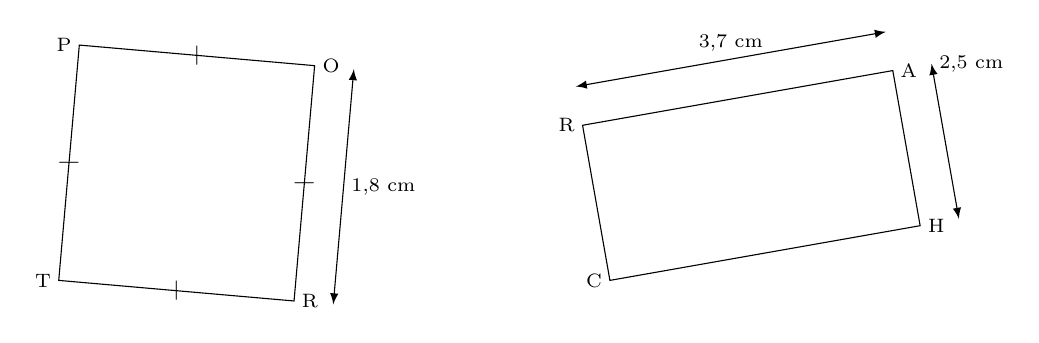
\begin{tikzpicture}

{\scriptsize
\begin{scope}[rotate=-5]
\coordinate[](T) at (0,0);
\coordinate[](R) at (3,0);
\coordinate[](O) at (3,3);
\coordinate[](P) at (0,3);

\tkzMarkRightAngle(T,R,O) ;
\tkzMarkRightAngle(R,O,P) ;
\tkzMarkRightAngle(O,P,T) ;
\tkzMarkRightAngle(P,T,R) ;

\draw (T)--node[sloped]{$|$} (R) --node[sloped]{$|$} (O) --node[sloped]{$|$} (P) --node[sloped]{$|$} cycle;
\draw[<->, >=latex] (3.5,0) -- (3.5,3);
\node[right] at (3.5,1.5) {1,8 cm} ;

%\node at (1.5,0) {$/$} ;
%\node at (3,1.5) {$/$} ;
%\node at (0,1.5) {$/$} ;
%\node at (1.5,3) {$/$} ;

\node[left] at (T) {T};
\node[right] at (R) {R};
\node[right] at (O) {O};
\node[left] at (P) {P};
\end{scope}


\begin{scope}[xshift=7cm, rotate=10]

{\scriptsize
\coordinate[](C) at (0,0);
\coordinate[](H) at (4,0);
\coordinate[](A) at (4,2);
\coordinate[](R) at (0,2);

\tkzMarkRightAngle(C,H,A) ;
\tkzMarkRightAngle(H,A,R) ;
\tkzMarkRightAngle(A,R,C) ;
\tkzMarkRightAngle(R,C,H) ;

\draw (C)-- (H) -- (A) -- (R) -- cycle;
\draw[<->, >=latex] (4.5,0) -- (4.5,2);
\node[right] at (4.5,2) {2,5 cm} ;
\draw[<->, >=latex] (4,2.5) -- (0,2.5) ;
\node[above] at (2,2.5) {3,7 cm} ;


\node[left] at (C) {C};
\node[right] at (H) {H};
\node[right] at (A) {A};
\node[left] at (R) {R};
}

\end{scope}
}
\end{tikzpicture}
 
\end{center}
}{2}
\end{exo}

%\begin{exo}{
%$MNOP$ est un rectangle et $QRST$ est un carré. Reproduis la figure avec tes instruments de géométrie en respectant les mesures.
%}{0}
%\end{exo}

\begin{exof}{ES81}{136}{1}
\end{exof}
	\begin{exol}{ES83}{112}{1}
	\end{exol}
		\begin{exol}{ES84}{113}{1}
		\end{exol}
			\begin{exol}{ES85}{113}{1}
			\end{exol}
				\begin{exol}{ES86}{113}{1}
				\end{exol}
					\begin{exol}{ES87}{113}{1}
					\end{exol}
						\begin{exol}{ES88}{113}{1}
						\end{exol}
							\begin{exol}{ES89}{114}{3}
							\end{exol}
								\begin{exof}{ES91}{140}{1}
								\end{exof}
									\begin{exof}{ES92}{141}{1}
									\end{exof}
										\begin{exol}{ES96}{115}{1}
										\end{exol}

										\begin{FLP}{137}{1}
\end{FLP}

\end{document}

